% STEP 1: Choose oneside or twoside. Use the 'draft' option a lot when writing.
\documentclass[english, oneside]{HYgradu}

\usepackage[utf8]{inputenc} % For UTF8 support. Use UTF8 when saving your file.
\usepackage{lmodern} % Font package
\usepackage{textcomp}
\usepackage[pdftex]{color, graphicx} % For pdf output and jpg/png graphics
\usepackage[pdftex, plainpages=false]{hyperref} % For hyperlinks and pdf metadata
\usepackage{fancyhdr} % For nicer page headers
%\usepackage{tikz} % For making vector graphics (hard to learn but powerful)
%\usepackage{wrapfig} % For nice text-wrapping figures (use at own discretion)
\usepackage{amsmath, amssymb} % For better math
\usepackage[sort,colon]{natbib} % For bibliography
\usepackage[footnotesize,bf]{caption} % For more control over figure captions

\renewcommand{\topfraction}{.75}
\renewcommand{\floatpagefraction}{.75}

\fussy % Probably not needed but you never know...

% OPTIONAL STEP: Set up properties and metadata for the pdf file that pdfLaTeX makes.
% But you don't really need to do this unless you want to.
\hypersetup{
    bookmarks=true,         % show bookmarks bar first?
    unicode=true,           % to show non-Latin characters in Acrobat’s bookmarks
    pdftoolbar=true,        % show Acrobat’s toolbar?
    pdfmenubar=true,        % show Acrobat’s menu?
    pdffitwindow=false,     % window fit to page when opened
    pdfstartview={FitH},    % fits the width of the page to the window
    pdftitle={},            % title
    pdfauthor={},           % author
    pdfsubject={},          % subject of the document
    pdfcreator={},          % creator of the document
    pdfproducer={pdfLaTeX}, % producer of the document
    pdfkeywords={something} {something else}, % list of keywords for
    pdfnewwindow=true,      % links in new window
    colorlinks=true,        % false: boxed links; true: colored links
    linkcolor=black,        % color of internal links
    citecolor=black,        % color of links to bibliography
    filecolor=magenta,      % color of file links
    urlcolor=cyan           % color of external links
}

% STEP 2:
% Set up all the information for the title page and the abstract form.
% Replace parameters with your information.
\title{Simulating the dynamics of supermassive black holes}
\author{Vili Oja}
\date{\today}
\level{Master's thesis}
\faculty{Faculty of Science}
\department{Department of Physics}
\address{PL 64 (Gustaf Hällströmin katu 2)\\00014 Helsingin yliopisto\\Finland}
\subject{Astronomy}
\prof{Professor Peter Johansson}
\censors{Professor Peter Johansson}{}{}
\depositeplace{}
\additionalinformation{}
\numberofpagesinformation{\numberofpages \ pages}
\classification{}
\keywords{Your keywords here}
\quoting{}

\begin{document}
\setlength{\parindent}{1cm}
\setlength{\parskip}{0cm}
% Generate title page.
\maketitle

% STEP 3:
% Write your abstract (of course you really do this last).
% You can make several abstract pages (if you want it in different languages),
% but you should also then redefine some of the above parameters in the proper
% language as well, in between the abstract definitions.
\begin{abstract}
Abstract goes here.
\end{abstract}

% Place ToC
\mytableofcontents



% -----------------------------------------------------------------------------------
% STEP 4: Write the thesis.
% Your actual text starts here. You shouldn't mess with the code above the line except
% to change the parameters. Removing the abstract and ToC commands will mess up stuff.
\setlength{\parindent}{.75cm}
\setlength{\parskip}{.6cm}
\chapter{Introduction}


\section{Discovery of black holes}

\section{History of black hole observations}
%miten eri aukkoja havaitaan, binääreissä pieniä aukkoja, keskustoissa suuria ja voidaan nähdä niiden vaikutus ympäröiviin tähtiin

\section{Aim of this thesis}

\chapter{Dynamical modelling of black holes}

\section{Black hole properties}

A black hole (BH) is defined as a region of spacetime for which the gravitational field is so strong that no objects or signals that carry information can escape from it. Black holes have the interesting property that their gravitational field is completely determined by the black hole's mass M, its angular momentum J, and its electric charge Q. This is known as the black hole uniqueness theorem or no-hair theorem, which states that all physical black hole solutions are completely characterized by the above-mentioned three parameters, and must satisfy the condition 
\begin{equation} \label{equ:bhunique}
M^2 - \left( \frac{J}{M} \right)^2 - Q^2 \geq 0 \ ,
\end{equation}
where we set $G = c = 1$ \citep{mazur:2001}.
Thus only by changing these variables can the properties of the black hole change. The physical reasoning for this uniqueness theorem is that the matter beyond the event horizon of a black hole cannot directly affect anything outside of it. Thus only the globally conserved characteristics, such as mass and angular momentum, survive and can be measured from the outside. The electric charge of black holes that appear in nature is most likely neutral, since having a non-neutral charge would require a very large imbalance in the amounts of protons and electrons that enter into the black hole, which is not a realistic scenario with normal matter.

Black holes can be divided into four distinct types based on these properties. Every black hole has mass, but the angular momentum and electric charge are not necessary.
\begin{table}[htb]
\centering
\caption{Different types of black holes}
\begin{tabular}{|c|c|c|}
\hline
 & Non-rotating ($J = 0$) & Rotating ($J \neq 0$) \\ \hline
Uncharged ($Q = 0$) & Schwarzschild & Kerr \\ \hline
Charged ($Q \neq 0$) & Reissner–Nordström & Kerr–Newman \\ \hline
\end{tabular}
\end{table}

The simplest type of black hole is created when an object of mass M becomes smaller than the radius
\begin{equation}
r_S = \frac{2GM}{c^2} \ .
\end{equation}
A black hole can be born in nature when massive a star dies and explodes in a supernova. As will be discussed in more detail in section \ref{sect:stellarholes}, massive stars can fuse matter up to iron, and an iron core is formed at the center of the star near the end of its lifetime. Once this core grows massive enough that the degeneracy pressure of electrons can no longer support its gravity, it will undergo catastrophic collapse. If the massive core collapses until it reaches the aforementioned radius, it will form a black hole. The radius is called the Schwarzschild radius, so named after the German astronomer Karl Schwarzschild, who found an exact solution for the Einstein field equations \citep{schwarzschild:1916}. Einstein field equations are the set of 10 equations in Albert Einstein's general theory of relativity that describe the fundamental interaction of gravitation as a result of spacetime being curved by mass and energy \citep{einstein:1915}. The surface at this radius is called the event horizon. Event horizons are mathematical surfaces, and they do not form any sort of physical barrier. An observer can fall inside the event horizon without any problem. The event horizon simply marks the limit at which not even light can escape the gravitational pull of the black hole.

There exists solutions that do not satisfy the condition given by equation \ref{equ:bhunique}, but these solutions are not stationary. In a stationary field the geometry does not change over time, but it can rotate, e.g. the Kerr solution. As will discussed soon, these non-stationary solutions are not really physical. This gives an upper limit to the angular momentum that a physical uncharged black hole can have. This limit can be expressed as the specific angular momentum 
\begin{equation} \label{equ:angularmomentum}
a = \frac{J}{Mc}
\end{equation}
or as the dimensionless spin parameter
\begin{equation}
a_* = \frac{Jc}{GM^2} \ .
\end{equation}
The parameter can range from 0, meaning that the hole does not spin, to almost 1, meaning that it spins as fast as possible for a given mass \citep{middleton:2016}.

If a black hole would have even larger angular momentum than allowed by these constraints, i.e. $a > 1$, it would mean that it actually would not be a black hole at all, since the event horizon would disappear due to the extreme rotation. 
%This is made clear by looking at equation \ref{equ:evenhorizons}, which describes the surfaces that event horizons occur at. If $\mu^2 < a^2$, the solutions for this equation are complex, which is said to mean that the actual event horizons disappear.
This would cause what is known as a naked singularity, meaning that a singularity that is normally contained within a black hole would be visible to an outside observer. The possible existence of such singularities in nature is uncertain but extremely unlikely. If they were to exist, they might cause fundamental problems for physics as we know it. We would be able to see matter condensed to infinite density, and we have no theories that can predict how spacetime works near such abnormalities. Normally this is not a problem, since they cannot be observed inside event horizons. However the cosmic censorship hypothesis suggests that naked singularities cannot be formed in nature from realistic initial conditions, which would avoid the problem altogether \citep{wald:1997}. An extremely rapid spin could prevent the collapse into a black hole thanks to the centrifugal forces. The object would have to lose enough of its angular momentum before it could collapse.

Astrophysical black holes that appear in nature are assumed to be most likely Kerr black holes. The normal matter that creates and feeds black holes contains roughly equal amounts of protons and electrons, so the overall electric charge is mostly neutral. But stars do spin around themselves, thus possessing angular momentum. Because of the conservation of angular momentum, the stellar remnant will spin around itself as well. Black holes can also gain more angular momentum via matter falling into them. Gas coming close to a black hole will form into an accretion disk around it. For the matter to be able to reach the black hole and fall into it, it must somehow lose some of its angular momentum. The total angular momentum of the disk must be conserved however, so the momentum has to move outwards in the disk. This happens due to collisions between the gas particles, which causes other particles to move slower and others faster. These slower moving particles then move closer to the black hole in the disk. Eventually the matter will fall within the event horizon, conferring its mass and remaining angular momentum to the black hole, speeding up the rotation of the black hole \citep{bhphysics}. Black holes are also capable of losing their angular momentum. One way for this to happen is through the emission of jets.

\subsection{The structure of a rotating black hole}

While Schwarzschild black holes have only the one event horizon and a point-like singularity in the middle, spinning black holes are far more complicated. All massive objects cause a space-time effect predicted by general relativity that is known as de Sitter precession or the geodetic effect. The presence of mass warps space-time, causing objects orbiting around the mass to precess slightly. In addition to this, spinning sources of gravity cause an additional effect called Lense-Thirring precession or frame-dragging. The massive object drags the surrounding spacetime with it as it spins, causing nearby particles and photons to rotate too, even if they did not have any angular momentum of their own to begin with. Both of these effects have been experimentally confirmed, for example by the Gravity Probe B mission. It measured the slight changes in the spin of gyroscopes aboard a satellite orbiting Earth, and confirmed that precession does indeed occur from both sources. The geodetic effect near Earth is around 170 times larger, so it can be measured more accurately \citep{everitt:2009}.

Thus the frame-dragging effect is significant only around very massive objects, like black holes that are rotating rapidly. At certain point this effect becomes so strong that any object, including light, \textit{must} spin along the rotation of the black hole. This limit is known as the stationary limit surface, and it is described in equation \ref{equ:statlimsurf}. The area inside this limit is called the ergosphere, so named after the Greek word for work. The ergosphere differs from the insides of an event horizon because particles that fall into it can actually still escape from this region. If a particle escapes from the ergosphere, it converts some of the black hole's rotation energy into it's own momentum \citep{grintro}. This lowers the angular momentum of the black hole, and the process could theoretically over time cause a rotating black hole to spin increasingly slower.

%This is called the Penrose process, and it is a possible explanation for some highly energetic astrophysical phenomena, such as gamma ray bursts. 
%TODO tarkenna tätä kappaletta

The Kerr metric is often presented in Boyer-Lindquist coordinates $(t, r, \theta, \phi)$ which are similar to spherical polar coordinates and are related to the Cartesian x,y,z-coordinates via the following transforms:
\begin{align*}
x &= \sqrt{r^2 + a^2} \mathrm{sin}\theta \mathrm{cos}\phi \\
y &= \sqrt{r^2 + a^2} \mathrm{sin}\theta \mathrm{sin}\phi \\
z &= r \mathrm{cos}\theta
\end{align*}
The variable $a$ is the same specific angular momentum as in the equation \ref{equ:angularmomentum}. The only true singularity (i.e. a singularity that exists no matter what coordinate system we choose) in the Kerr metric occurs when $r=0$ and $\theta = \pi/2$ \citep{grintro}. It is easy to see that in Cartesian coordinates this corresponds to a flat ring in the equatorial plane with the radius of $a$. So rotating black holes do not have a point singularity, but a ring singularity instead.

In addition there exists coordinate singularities (i.e. singularities we can get rid of if we choose our coordinates differently) as well. These singularities occur on the surfaces
\begin{equation} \label{equ:evenhorizons}
r_\pm = \mu \pm \sqrt{\mu^2 - a^2}
\end{equation}
which describe the event horizons of the black hole, and on the surfaces
\begin{equation} \label{equ:statlimsurf}
r_{S \pm} = \mu \pm \sqrt{\mu^2 - a^2 \mathrm{cos}^2 \theta}
\end{equation}
which describe the stationary limit surfaces of the black hole. Here $\mu = \frac{GM}{c^2}$. 

In figure \ref{fig:KerrHole} one can see the different surfaces of a spinning black hole and their approximate shapes. The surfaces mostly resemble axisymmetric ellipsoids, flattened along the rotation axis. Although the outer limit of the ergosphere changes its shape as the spinning gets faster, resembling a pumpkin-shape at nearly maximal spins. It however always touches the outer event horizon at the poles. The inner horizon and stationary limit surface also touch at the poles. On the equatorial plane the inner stationary limit surface also coincides with the ring singularity.

\begin{figure}
\centering
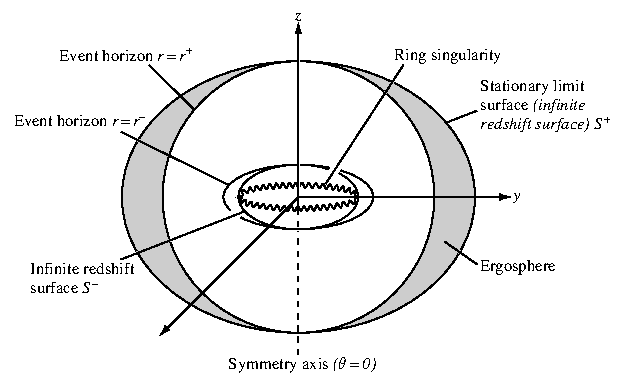
\includegraphics[width=\textwidth]{../images/kerrhole.pdf}
\caption{Diagram showing the structure of a Kerr black hole. It shows the inner and outer ergospheres and event horizons, and the ring singularity in the middle. This kind of black hole has non-zero spin. If the spin was 0 we would have a Schwarzschild black hole instead.
(Figure adapted from \citealt{grintro})}
\label{fig:KerrHole}
\end{figure}

%TODO

%Kahdenlaista frame draggingia Lense-Thirring efekti pyörivillä

%mainitse Eddingtonin luminositeetti yms jutut? Muuttaa valtavasti massaa energiaksi.

%mainitse miten voi menettää massaa?
\newpage
\section{Different types of black holes}

Mass is the only quantity that all black holes have for certain, so it makes sense to classify them by their mass. The black holes are usually put into three different categories. The reason for this kind of distinction is that the different mass black holes are found in very different kinds of environments and have varying formation histories. The black holes are also detected through the different kinds of phenomena that they cause. %TODO vähennä different käyttöä
The mass limits for the categories are not exact, but typically stellar mass black holes (SBH) are below $10^2 \ M_\odot$, intermediate mass black holes (IMBH) are between $10^2$ and $10^5 \ M_\odot$, and supermassive black holes (SMBH) are above $10^5 \ M_\odot$ \citep{bhphysics}.

%kerro eri kohissa et miten voi havaita, mitä eri ilmiöitä nää ehkä synnyttää
%kerro miten syntyvät, massarajoja, tähden kokonaismassa on eri kuin ytimen massa, joka kertoo voiko syntyä musta aukko

\subsection{Stellar mass black holes} \label{sect:stellarholes}

Stellar mass black holes are born from collapsing massive stars. During their active life, stars stay in hydrostatic equilibrium due to the gravitational pull of the matter making up the star, and the outward thermal pressure caused by the nuclear reactions in the star's core. At the end of a massive star's lifespan, the hydrogen in the core will have fused into helium. This leads to hydrogen forming a shell around the helium core, and hydrogen fusion will continue there, which is known as shell burning. The helium formed in the shell will accrete into the core, causing the core to grow hotter and denser. Once the core is has grown enough, the helium will start to fuse as well. This same process will happen for heavier elements as well, until the star will have several shells of different elements, as illustrated in figure \ref{fig:FusionShells}.

\begin{figure}[h!tb]
\centering
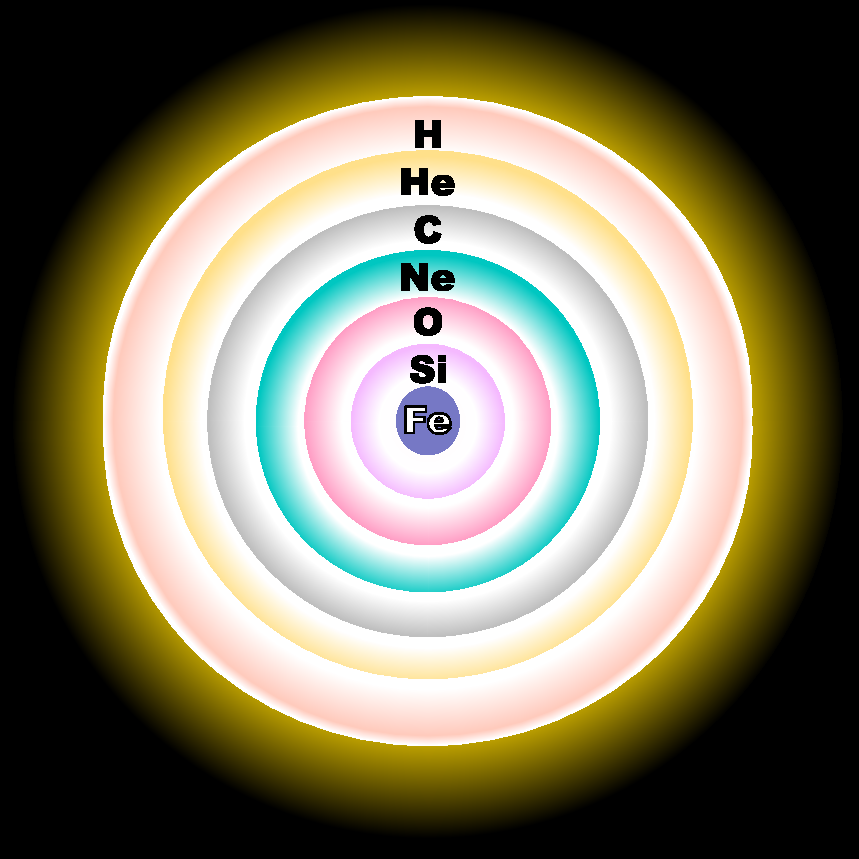
\includegraphics[width=\textwidth]{../images/FusionShells.pdf}
\caption{A simplified cross-section of a massive, evolved star. As the star starts fusing heavier and heavier elements, new shells will form around the previous ones, until the core becomes iron, which cannot go through fusion without losing energy.
(\copyright \ User:Rursus / Wikimedia Commons / CC-BY-SA-3.0)}
\label{fig:FusionShells}
\end{figure}

Iron and nickel have the highest binding energies of all the elements, meaning that lighter elements release energy through fusion, but reactions producing heavier elements require additional energy. The star cannot fuse any more matter in its core, and thus the supporting pressure drops, causing the star to implode under its own gravity. Iron being the final product in stars causes what is known as the iron peak in the abundance of chemical elements. Iron is one of the most common metals in the universe, as seen in figure \ref{fig:IronPeak}. One can also see that certain other elements such as carbon, oxygen, neon, etc. are more abundant than other elements near their mass. This too is the result of stellar nucleosynthesis, where these elements are created through fusion with helium nuclei, which are known as alpha particles. Due to this, all of these so called alpha elements have a mass number that is a multiple of four.

What happens next depends on the mass of the star. For the star to be able to even reach this stage, it needs to be initially over around 8 solar masses. Otherwise it does not have enough mass to fuse the heavier elements, and it will gradually expand its atmosphere into a planetary nebula, leaving behind a white dwarf. In more massive stars, the iron core will exceed the Chandrasekhar limit of around 1.4 solar masses, which describes the upper limit for the mass of a stable white dwarf. Stars above this $\sim$8 solar mass threshold but below $\sim$20 solar masses explode in supernovae and leave behind neutron stars. If the initial mass of the star is even higher than that, the stellar core is too massive to not collapse into a black hole \citep{woosley:2002}. The actual mass limit is the Tolman–Oppenheimer–Volkoff limit, which gives the upper bound for a cold, non-rotating neutron star, and is about 2.2 solar masses. These limits have to do with the properties of the degenerate matter that dense stellar remnants are made of. While main sequence stars stay in hydrostatic equilibrium thanks to thermal pressure, stellar remnants resist collapse through degeneracy pressure. White dwarfs and neutrons stars can be modelled as a Fermi gas, which is the quantum mechanical equivalent of an ideal gas. The Pauli exclusion principle states that identical fermions cannot occupy the same quantum state within a quantum system simultaneously. Thus there exists a sort of interaction or pressure between the particles in a Fermi gas that keeps them separate, even at absolute zero temperature. This manifests as a degeneracy pressure that resists further gravitational collapse. In white dwarfs the electron degeneracy pressure is what keeps the object in an equilibrium. Past the Chandrasekhar limit the electrons will combine with protons to form neutrons, forming a remnant made of degenerate neutron matter. Neutron stars are then supported by the degenerate neutron pressure. For stellar remnants more massive than the Tolman–Oppenheimer–Volkoff limit, the gravitational pull will exceed even the degenerate pressure, causing the remnant to collapse into a black hole. This also gives a lower limit for the mass of new black holes that form through stellar collapse.

\begin{figure}
\centering
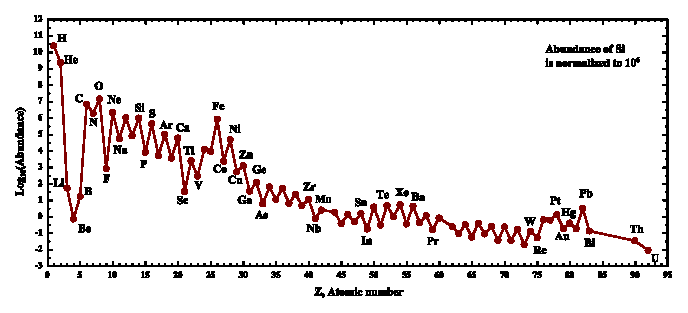
\includegraphics[width=\textwidth]{../images/SolarSystemAbundances.pdf}
\caption{Diagram illustrating the abundancies of different elements in our solar system. Iron is the final product of fusion in stars, causing it to be very abundant in the universe thanks to its production in stars before they explode. The abundant alpha elements are also clearly noticeable.
(\copyright \ User:MHz\textasciigrave as / Wikimedia Commons / CC-BY-SA-3.0)}
\label{fig:IronPeak}
\end{figure}

One way stellar mass black holes have been observed is in X-ray binaries. These kinds of binaries were discovered through the detection of highly energetic X-ray sources, having luminosities with the same magnitude as the theoretical maximum luminosity from matter accreting onto a black hole, assuming simple spherical accretion. This is called the Eddington limit, and it will be discussed more later on. This combined with their low timescale variability (down to milliseconds) lent support for a model where the X-rays are produced by matter from a star accreting onto a compact object. The mass of the compact object $M_x$ can be estimated by measuring the orbital period $P$, radial velocity amplitude $K$, the mass of the companion star $M_c$, and the inclination angle $i$. Inclination is important because of the mass-inclination degeneracy. Measuring the true orbital velocity of a star depends on its inclination, and thus measuring the mass of the star star also depends on it. The inclination can be constrained for example by tracking and modelling how the brightness of the star varies along the orbit \citep{kerkwijk:2011}. These are used in the mass function equation 
\begin{equation}
f(M_x) = \frac{K^3 P}{2 \pi G} = \frac{M_x^3 \mathrm{sin}^3 i}{(M_x + M_c)^2}
\end{equation}
which tells the lower limit for $M_x$ \citep{casares:2007}. The key factor in the equation is $M_c$ which can have a lot of uncertainty. The reason that the mass of the central object is interesting is that both neutron stars and black holes can produce X-ray radiation. Matter accreting onto the objects heats up in the accretion disc due to the particles colliding with each other. The matter can reach temperatures of millions of degrees and radiates away its potential energy as X-rays. With neutron stars, infalling matter can also actually hit the surface of the object, heating up upon impact to emit X-rays. If the mass can be measured to be well above the aforementioned Tolman–Oppenheimer–Volkoff limit, other objects than black holes can be quite safely ruled out.

%puhu muista tavoista havaita, värihommaa?
%neutronitähdissä voi olla flareja

%fuusiokartta, raudasta ei pääse eteenpäin, iron peak

%observable in x-ray compact binary systems

\subsection{Intermediate mass black holes}

Intermediate mass black holes are much more elusive compared to both their more massive and lighter companions. We have only very few good candidates and their formation is not fully understood. Learning more about both the birth and evolution of intermediate mass black holes is an important topic, as it allows us to learn more about how lighter black holes gain mass and form supermassive black holes, which in turn is a key element in understanding the formation and evolution of galaxies.

One way for black holes to grow in mass is through the accretion of gas. Matter that accretes onto a black hole forms a disk and must lose its angular momentum before it can end up in the black hole. The matter particles can collide with each other, creating heat and effectively moving the angular momentum outwards, so the inner parts of the disk can fall closer into the black hole. The heat is radiated away, usually in the form of X-rays. This process creates radiation pressure that resist more matter falling into the black hole. The radiation increases as more matter accretes onto the hole, and the limit where the outward radiation force and the inward gravitational force are balanced is called the Eddington luminosity or Eddington limit. This limit, assuming spherical accretion, is given by
\begin{equation}
L_{Edd} = \frac{4 \pi c G M m_p}{\sigma_T} \simeq 1.26 \left( \frac{M}{M_\odot} \right) W = 3.2 \times 10^4 \left( \frac{M}{M_\odot} \right) L_\odot \ ,
\end{equation}
where $c$ is the speed of light, $G$ is the gravitational constant, $M$ is the mass of the black hole, $m_p$ is the proton mass, and $\sigma_T$ is the Thomson scattering cross-section for an electron. The Thomson cross-section describes the effective area for photon interactions for a free charged particle. Assuming there are no other effects which affect the accretion rate, this limit gives the maximum rate at which black holes can grow solely through spherical accretion. 

A so called `seed' black hole with a mass around $10^6 M_\odot$ would require over 0.5 Gyr to grow into a $10^9 M_\odot$ supermassive black hole, given it constantly grows at Eddington rate. Due to this fact, the observed existence of supermassive black holes of $10^9 M_\odot$ when the universe was around 1 Gyr old implies that these seed black holes must have formed at redshifts larger than 10. In such a young universe there are several ways that intermediate mass black holes could form \citep{mezcua:2017}. These methods are illustrated in figure \ref{fig:imbhs}.

\begin{figure}
\centering
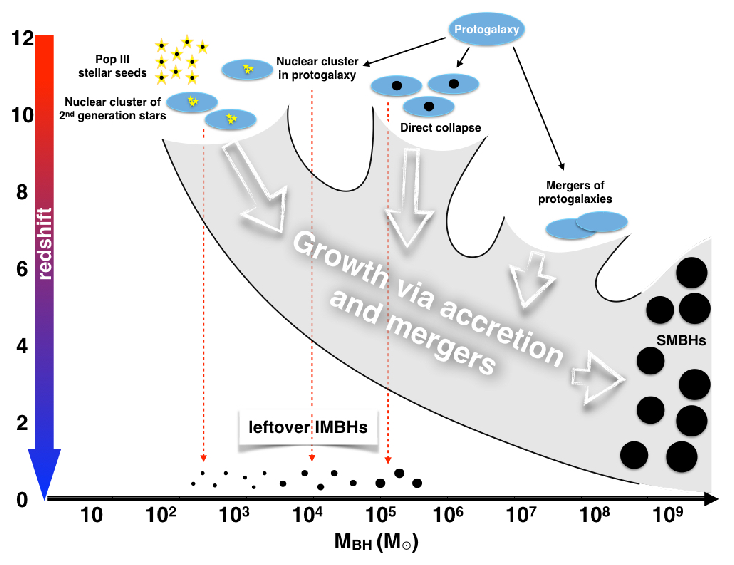
\includegraphics[width=\textwidth]{../images/imbhs.pdf}
\caption{Different methods of birth for seed intermediate mass black holes. These include collapse of Pop III stars, mergers in dense stellar clusters, and direct collapse of gas in protogalaxies. Some black holes will grow to be supermassive, but some will stay in their intermediate state to this day.
(Figure adapted from \citealt{mezcua:2017})}
\label{fig:imbhs}
\end{figure}

One way for these kinds of black holes to form could be through massive Population III stars. These stars formed early in the universe and thus they had very low metallicities, since heavy elements had not yet formed. Low metallicity allowed these stars to grow very large. This can be explained with how metallicity affects the cooling of gas clouds. 
Here the most relevant cooling processes are two-body radiative cooling processes. Free-free emissions happen due to acceleration of electrons when they encounter atomic nuclei. In free-bound emissions an electron recombines with an ion and emits a photon to cool down the gas. Bound-free emission happens when an electron collides with an atom or ion and ionizes it. In bound-bound emissions atoms are excited via collisions, and they emit photons as they decay back to the ground state. Metals have more possible energy states, so more metals means that these processes can happen more often, thus allowing for more efficient cooling.
Jeans mass gives the limit for the size of a symmetrical, non-rotating gas cloud before it will collapse under its own gravity. The limit comes from when the cloud's thermal energy and gravitational potential are in equilibrium. The mass can be calculated by
\begin{equation}
M_J = \left( \frac{5 k T}{G \mu m} \right)^{3/2} \left( \frac{3}{4 \pi \rho} \right)^{1/2} \ ,
\end{equation}
where $k$ is the Boltzmann's constant, $G$ the gravitational constant, $T$ the temperature of the gas, $\rho$ the density of the gas, $\mu$ the mean molecular weight, and $m$ the mass of a particle comprising the gas. So the hotter and thinner the gas cloud is, the more massive it has to be for it to collapse. 

At the start of the contraction, the cloud undergoes isothermal collapse. Meaning that the density increases but the temperature can stay approximately constant thanks to cooling. This can allow the cloud to fragment, as isothermal collapse causes the Jeans mass to decrease, allowing the cloud to start collapsing around small internal density inhomogeneities. As the density increases, the cloud becomes more optically thick and the temperature will start to rise as well. This adiabatic collapse will cause the cloud to start heating up into a protostar. If cooling is inefficient to begin with, like in metal-poor clouds made of molecular hydrogen, the isothermal phase can be quite short, decreasing fragmentation, allowing the stars to become very big, and Pop III stars can exceed 200 solar masses.

These stars can also retain their mass as they exhibit weaker stellar winds compared to more metal-rich stars. This is because radiation pressure on many spectral lines is the main mechanism behind winds in massive stars. Hydrogen and helium have only few relevant lines, so metal lines are the major reason for strong stellar winds \citep{vink:2001}. When these stars collapse in a similar manner to lower mass stars, they could then form black holes with masses of several hundred $M_\odot$. These kinds of black holes would still be relatively light, requiring super-Eddington accretion rates to reach the observed masses at around redshift 6.

To circumvent this problem, the seed black holes would need to be more massive from the start. Black holes could also form inside the first protogalaxies by direct collapse of gas. The formation of these black holes would require a rapid inflow of dense gas. The gas must have minimal angular momentum so that it does not form a disk structure to support itself. In addition, to prevent fragmentation, atomic hydrogen, not molecular hydrogen, must dominate the cooling process, making it extremely inefficient. In this kind of environment the gas could form supermassive stars with masses of $10^5 M_\odot$, which could collapse into black holes of $10^4 - 10^5 M_\odot$. Another prediction for their formation is through multiple mergers in dense stellar clusters. In a dense region of stars, multiple stellar mergers can cause the formation of supermassive stars that can collapse into black holes of $10^2 - 10^4 M_\odot$ \citep{mezcua:2017}.

To figure out whether intermediate mass black holes exist or not, we need to measure the mass of candidate black holes. The most accurate way to probe the mass is through stellar or gas dynamics. i.e. observing the movements of objects around the black hole, and measuring the mass of the central object based on their orbits. Although with our current instruments this method only works for relatively nearby objects. A black hole of $10^5 M_\odot$ has a sphere of influence of about 0.5 pc, and cannot be resolved beyond a megaparsec. Sphere of influence describes the area around a black hole where its gravitational potential dominates the potential of the surrounding galaxy. It is defined with the equation 
\begin{equation}
r_h = \frac{G M_{BH}}{\sigma^2} \ ,
\end{equation}
where $G$ is the gravitational constant, $M_{BH}$ the mass of the black hole, and $\sigma$ the velocity dispersion of the stars in the surrounding bulge.
In addition to kinematics, radiation signatures such as X-ray and radio emissions can be used to ascertain whether an object is a black hole and what its mass is. One of the best current candidates for an intermediate mass black hole is the central object in the globular cluster G1. Both X-ray and radio emissions have been detected there, and photometric and kinematic observations have given an estimate for a black hole with a mass of around $1.8 \times 10^4 M_\odot$ \citep{gebhardt:2005}. One can obtain the mass through these measurements by calculating the full line-of-sight velocity distribution (LOSVD), and using this velocity to estimate the central mass.

\subsection{Supermassive black holes}

Supermassive black holes are the sources of some of the most energetic phenomena in the known universe, thus we have been able to detect their presence despite their relative scarcity and distance. They are found in the centers of galaxies, and it is nowadays generally accepted that supermassive black holes are present in practically every massive galaxy with a bulge component \citep{kormendy:2013}. What would eventually become the first candidates for supermassive black holes were discovered when very luminous radio sources were observed in the 1960s \citep{greenstein:1964}. First thought to be stars, their luminosities, redshifts, and short timescale variabilities made it quite clear that they were something else, hence they were dubbed quasi-stellar objects, or quasars. It was later proposed that matter falling onto a massive compact object could explain the phenomenon.

\begin{figure}[h!tb]
\centering
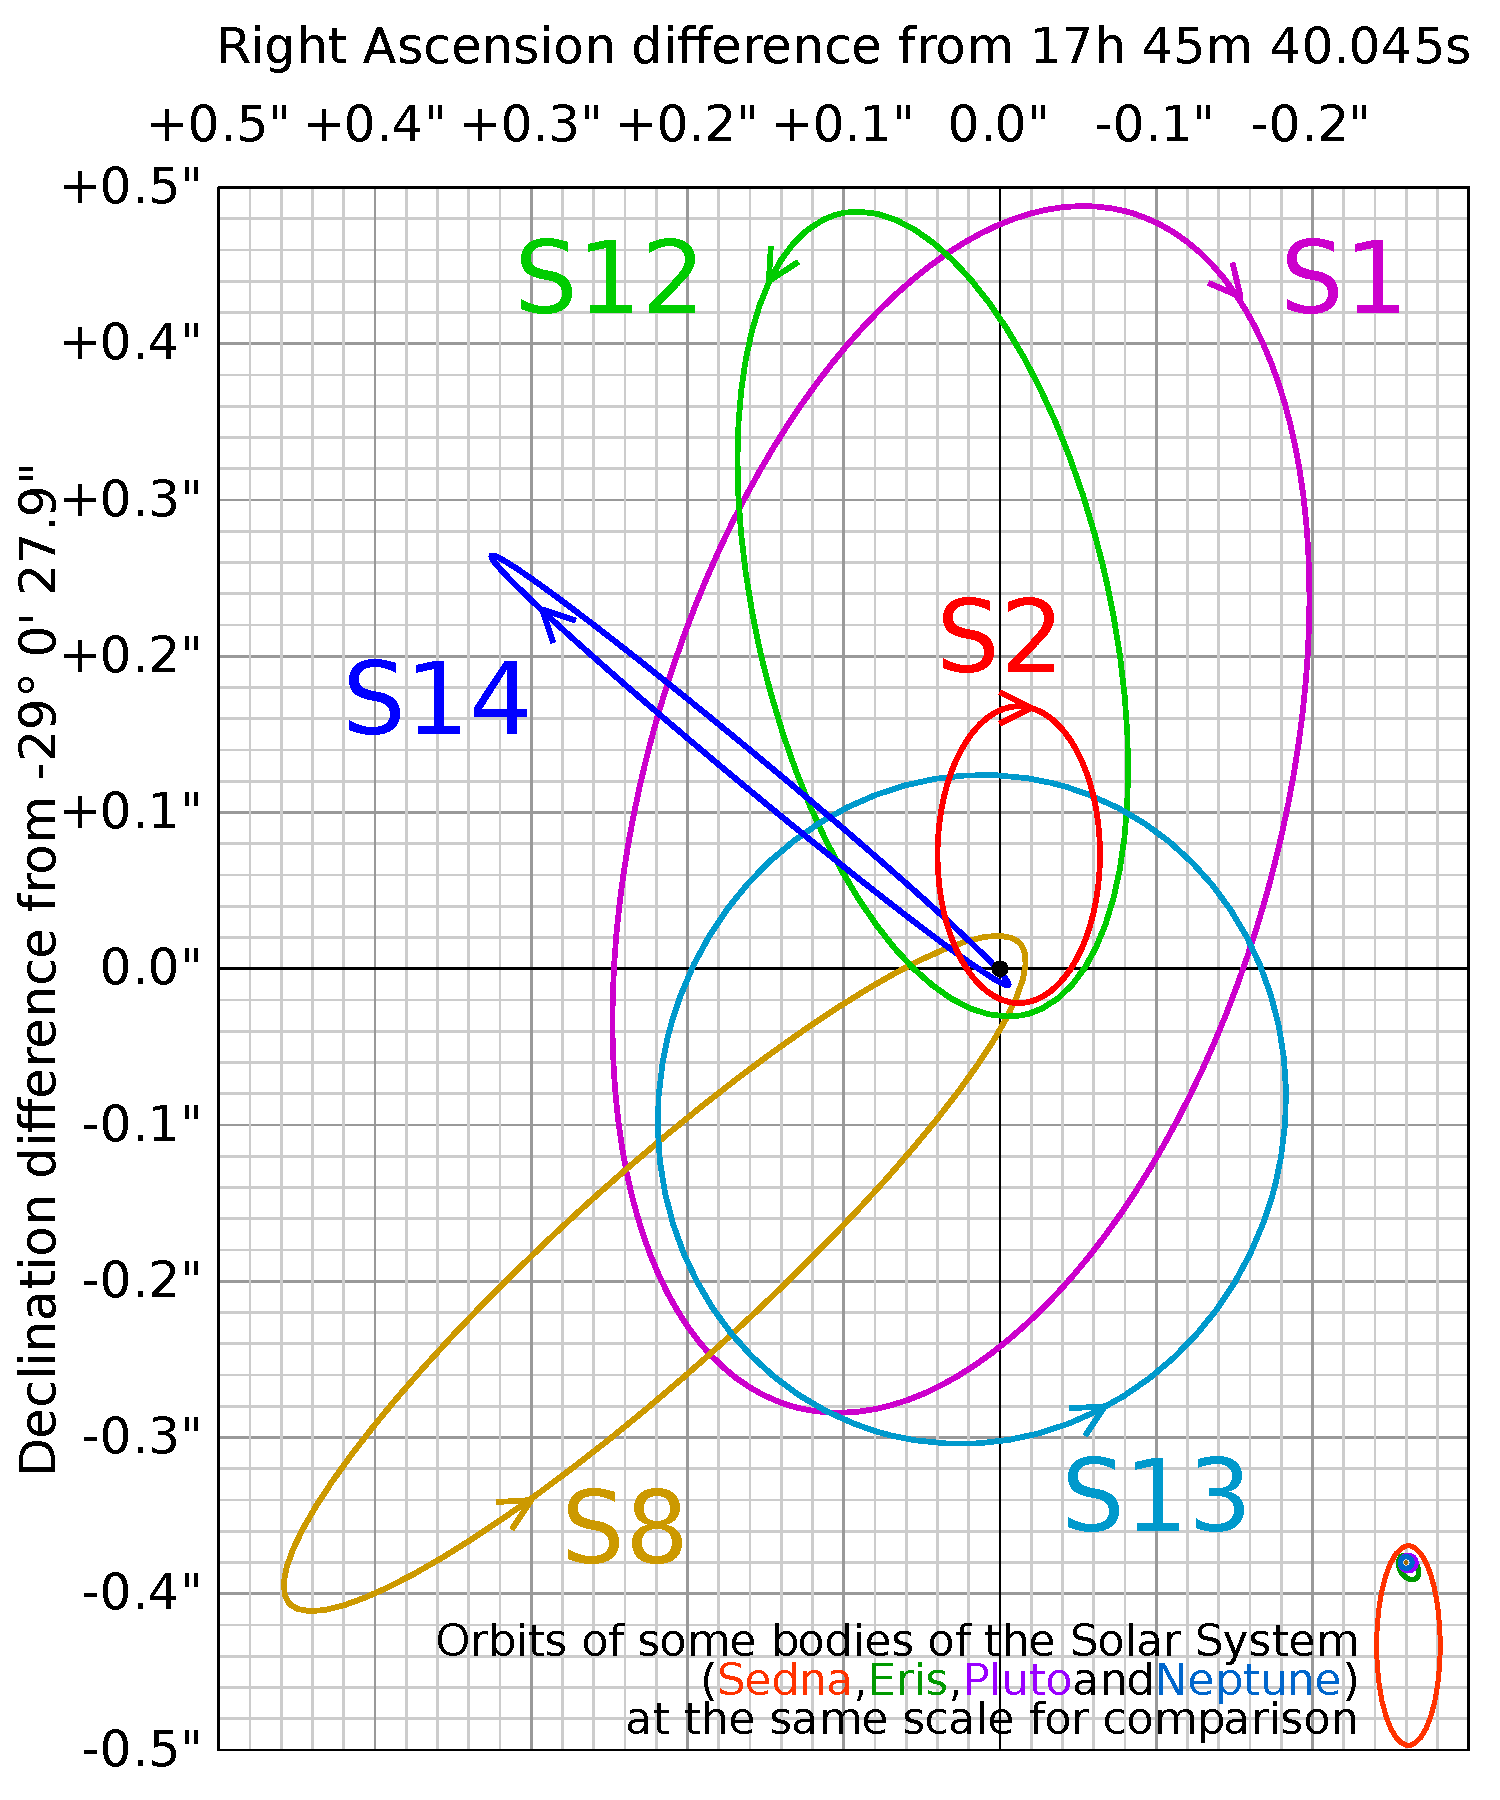
\includegraphics[width=\textwidth]{../images/MilkyWaySMBH.pdf}
\caption{Illustration of the well-determined orbits of 6 stars around Sagittarius A* in the galactic centre of our Milky Way. The star S2 has an orbital period of about 16 years, and has given us the most accurate estimate for the black hole mass to date. The data is based on \cite{eisenhauer:2005}.
(\copyright \ User:Cmglee / Wikimedia Commons / CC-BY-SA-3.0)}
\label{fig:MilkyWayBH}
\end{figure}

On top of spectroscopic measurements, the high resolution of the Hubble Space Telescope (HST) has enabled us to do dynamical measurements of galaxies and their massive black holes, meaning that we can track the movements of stars in these distant galaxies. In addition to HST, thanks to advances in adaptive optics, ground based observations have given us the best proof for a supermassive black hole at the center of our own galaxy. The galactic center is only around 8.1 kpc away \citep{eisenhauer:2018}, so individual stars can be resolved and their orbits determined. In figure \ref{fig:MilkyWayBH} orbits of 6 stars orbiting around the galactic center are visualized. Based on the orbit of the star S2, there must be a mass of around $4 \times 10^6 M_\odot$ at the center of the galaxy, and it must be located inside the radius of around 120 AU, otherwise the star would collide with the central mass \citep{kormendy:2013}. This rules out the possibility of the central mass being a large group of smaller masses, and makes a singular, massive central object the most likely scenario.

Supermassive black holes are believed to play an important role in the formation and evolution of galaxies. The mass of the central black hole correlates with the properties of the host galaxy and central bulge that contains it. The first of these correlations to be observed was the $M_{BH} - L_{bulge}$ correlation. The correlation between the black hole mass and the luminosity of the bulge has been tested on many galaxies, and it seems to be very consistent. The luminosity of the bulge is dependent on the mass of the bulge, but the correlation between the explicitly measured mass of the bulge and the black hole mass has also been tested and observed. This $M_{BH} - M_{bulge}$ relation is expressed by
\begin{equation}
\mathrm{log} (M_{BH}/M_{\odot}) = 1.12 \  \mathrm{log} (M_{bulge}/ 10^{11} M_{\odot}) + 8.2 \ ,
\end{equation}
and it has been found to be accurate for many galaxies \citep{haring:2004}.

One way to measure the mass of the bulge is by calculating its virial mass. The virial theorem relates the kinetic energy of a stable to system with its potential energy. In astrophysics the common use of this relation is to relate the gravitational potential energy of a system with its kinetic energy. The virial mass of a bulge can be calculated with the equation
\begin{equation}
M_{bulge} = \frac{k r_e \sigma^2_e}{G} \ ,
\end{equation}
where $k$ is a scaling factor, $r_e$ is the effective radius, $\sigma_e$ is the velocity dispersion inside the effective radius, and $G$ is the gravitational constant \citep{marconi:2003}. The velocity dispersion of the galaxy has been used in these previous correlations, but there seems to be a correlation between the black hole mass and the velocity dispersion itself. This $M_{BH} - \sigma$ relation is given by
\begin{equation}
\mathrm{log} \ M_{BH} = 4.8 \ \mathrm{log} \ \sigma - 2.9 \ , 
\end{equation}
and it has been found to be highly accurate for many galaxies \citep{ferrarese:2000}.
A tight $M_{BH} - \sigma$ correlation is important on a practical level since it allows for good estimates of the black hole mass from relatively easy measurements, and it also implies a link between the growth of the black hole and formation of the bulge \citep{kormendy:2013}.

%TODO
%korrelaatio massan ja ytimen ominaisuuksien välillä?
%miten havaitaan, AGN, kinematiikka
%syntyy keskimassaisista
%M-sigma relaatio?

\section{Newtonian dynamics}

\subsection{Two-body problem}

Solving the Newtonian two-body problem, i.e. determining the motions of two particles interacting only with each other through gravity, is extremely useful. It allows solving the behaviour of two essentially isolated objects, such as a binary star system. It for example also enables us to calculate the masses of two objects that are observed to be interacting with each other if their orbits are known.

Let us assume we have a mass $m_1$ situated at position vector $\mathbf{r}_1$, and a mass $m_2$ at position vector $\mathbf{r}_2$. If the first mass exerts a force $\mathbf{f}_{21}$ on the second mass, by Newton's third law the second object exerts an equal and opposite force, $\mathbf{f}_{12} = -\mathbf{f}_{21}$, on the first object. The masses and their positions are illustrated in figure \ref{fig:2BodyProb}. If these two objects are the only objects in the system, their equations of motion are
\begin{align}
m_1 \mathbf{\ddot{r}}_1 &= -\mathbf{f} \label{equ:eom1} \\
m_2 \mathbf{\ddot{r}}_2 &= \mathbf{f} \label{equ:eom2} \ ,
\end{align}
where $\mathbf{f} = \mathbf{f}_{21}$.

\begin{figure}[h!tb]
\centering
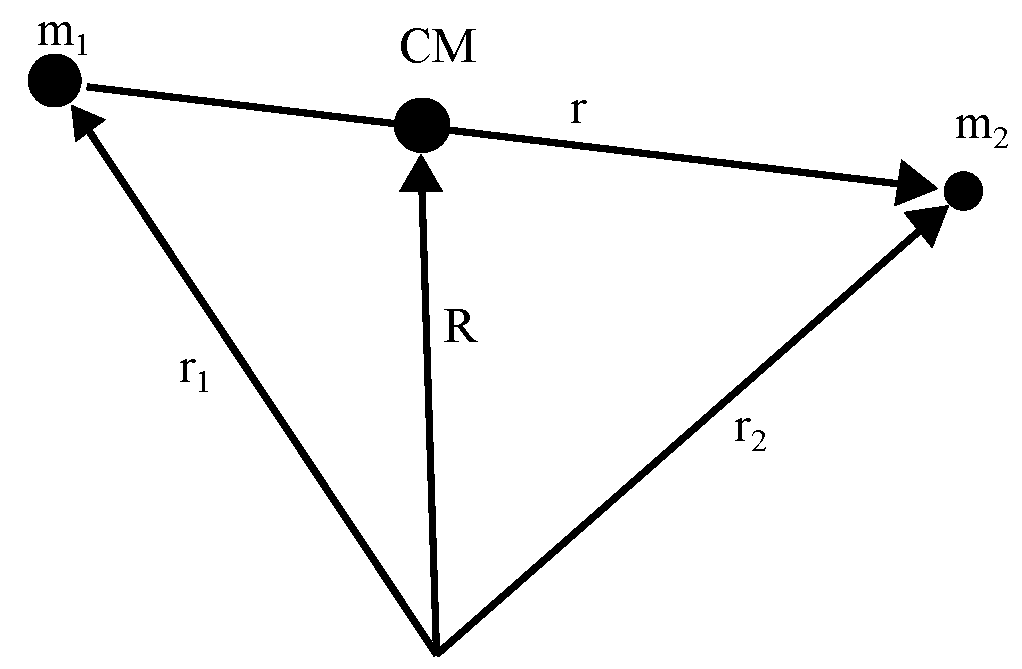
\includegraphics[scale=0.5]{../images/2bp.pdf}
\caption{The position vectors $\mathbf{r}_1$ and $\mathbf{r}_2$ point to the masses $m_1$ and $m_2$ respectively. $\mbox{$\mathbf{r} = \mathbf{r_2} - \mathbf{r_1}$}$ is their relative displacement vector, and $\mathbf{R}$ is the position vector of the center of mass of the system.}
\label{fig:2BodyProb}
\end{figure}

We can first get an equation describing the motion of the center of mass of the system by adding the equations \ref{equ:eom1} and \ref{equ:eom2} together. The position vector of the center of mass is
\begin{equation}
\mathbf{R} = \frac{m_1 \mathbf{r}_1 + m_2 \mathbf{r}_2}{m_1 + m_2}
\end{equation}
and by performing the addition we get
\begin{equation}
m_1 \mathbf{\ddot{r}}_1 + m_2 \mathbf{\ddot{r}}_2 = (m_1 + m_2) \mathbf{\ddot{R}} = \mathbf{f} - \mathbf{f} = 0 \ .
\end{equation}
This gives us that
\begin{equation}
\mathbf{\ddot{R}} = 0 \ ,
\end{equation}
which shows that the velocity of the center of mass is constant. So the position of the center of mass can be determined at all times from the initial positions and velocities. We can denote the relative displacement vector of the two masses with $\mbox{$\mathbf{r} = \mathbf{r_2} - \mathbf{r_1}$}$. Together with this and the center of mass vector, we can write
\begin{align}
\mathbf{r_1} &= \mathbf{R} - \frac{m_2}{m_1 + m_2}\mathbf{r} \\
\mathbf{r_2} &= \mathbf{R} + \frac{m_1}{m_1 + m_2}\mathbf{r}
\end{align}
Substituting these equations into \ref{equ:eom1} and \ref{equ:eom2}, we can see that both yield 
\begin{equation}
\mu \mathbf{\ddot{r}} = \mathbf{f} \ , \label{equ:eom3}
\end{equation}
where
\begin{equation}
\mu = \frac{m_1 m_2}{m_1 + m_2}
\end{equation}
is called the reduced mass. Thus we have effectively converted the two-body problem of masses $m_1$ and $m_2$ into a one-body problem of the reduced mass $\mu$. The situation is now simpler since we do not have to inspect the movement of two separate particles, but only the movement of one particle with respect to the other particle.

In the case of celestial objects, the force affecting the masses is gravity. The Newtonian gravitational force that the first object exerts on the second object is given by
\begin{equation}
\mathbf{f} = -\frac{G m_1 m_2}{r^3} \mathbf{r}
\end{equation}
where $\mathbf{r}$ is the aforementioned displacement vector and $G$ is the gravitational constant. Substituting this into equation \ref{equ:eom3} gives us
\begin{equation}
\frac{m_1 m_2}{m_1 + m_2} \mathbf{\ddot{r}} = -\frac{G m_1 m_2}{r^3} \mathbf{r}
\end{equation}
which gives us the equation of motion
\begin{equation}
\mathbf{\ddot{r}} = -\frac{G M}{r^3} \mathbf{r} \label{equ:eomgravity}
\end{equation}
where $M = m_1 + m_2$ is the total mass of the system.

\subsection{Equation of the orbit}

The derivation for the Keplerian equation of orbit is done following \cite{bt-galdyn}. The position vector can be expressed as
\begin{equation}
\mathbf{r} = r \hat{\mathbf{e}}_r \ ,
\end{equation}
where $\hat{\mathbf{e}}_r$ is a direction vector. The gravitational field in the equation of motion can be expressed as
\begin{equation}
g(r) = -\frac{G M}{r^2} \ ,
\end{equation}
so the equation of motion becomes
\begin{equation}
\frac{\mathrm{d}^2 \mathbf{r}}{\mathrm{d} t^2} = g(r) \hat{\mathbf{e}}_r \ .
\end{equation}
Since the cross product of a vector with itself is zero, we can see that
\begin{equation}
\frac{\mathrm{d}}{\mathrm{d} t} \left( \mathbf{r} \times \frac{\mathrm{d} \mathbf{r}}{\mathrm{d} t} \right) = \frac{\mathrm{d} \mathbf{r}}{\mathrm{d} t} \times \frac{\mathrm{d} \mathbf{r}}{\mathrm{d} t} + \mathbf{r} \times \frac{\mathrm{d}^2 \mathbf{r}}{\mathrm{d} t^2} = 0 + r \hat{\mathbf{e}}_r \times g(r) \hat{\mathbf{e}}_r = 0 \ ,
\end{equation}
thus $\mathbf{r} \times \mathbf{\dot{r}}$ is some constant vector, which we can denote with for example $\mathbf{L}$. This is simply the angular momentum per unit mass. It is a constant vector, and therefore the movement of the orbiting objects must take place in a plane. Limiting the movement to two dimensions simplifies the situation, and we can use plane polar coordinates $(r, \theta)$ where the center of attraction is at $r = 0$ and $\theta$ is the azimuthal angle in the plane. We can now find the equations of motions for the system in these coordinates by forming the Lagrangian per unit mass, which is
\begin{equation}
\mathcal{L} = K - V = \frac{1}{2} \mathbf{v}^2 - \Phi (r) = \frac{1}{2} \left[ \dot{r}^2 + (r \dot{\theta})^2 \right] - \Phi (r) \ ,
\end{equation}
where $\Phi$ is the gravitational potential and $g(r) = -\mathrm{d} \Phi / \mathrm{d} r$. Writing out the Lagrange equations gives us the equations of motion, which are
\begin{align}
\frac{\mathrm{d} }{\mathrm{d} t} \left( \frac{\partial \mathcal{L}}{\partial \dot{r}} \right) - \frac{\partial \mathcal{L}}{\partial r} &= \ddot{r} - r \dot{\theta}^2 + \frac{\mathrm{d} \Phi}{\mathrm{d} r} = 0 \label{equ:leom1} \\
\frac{\mathrm{d} }{\mathrm{d} t} \left( \frac{\partial \mathcal{L}}{\partial \dot{\theta}} \right) - \frac{\partial \mathcal{L}}{\partial \theta} &= \frac{\mathrm{d}}{\mathrm{d} t} (r^2 \dot{\theta}) = 0 \label{equ:leom2} \ .
\end{align}
Equation \ref{equ:leom2} implies that $r^2 \dot{\theta}$ is a constant, which we can denote with $L$. And this is actually the same $L$, angular momentum per unit mass, as before. So this equation is a restatement of the conservation of angular momentum. We can use it to replace time with angle as the independent variable in equation \ref{equ:leom1}. Equation \ref{equ:leom2} implies that
\begin{equation}
\frac{\mathrm{d}}{\mathrm{d} t} = \frac{L}{r^2} \frac{\mathrm{d}}{\mathrm{d} \theta} \ ,
\end{equation}
so equation \ref{equ:leom1} becomes
\begin{equation}
\frac{L^2}{r^2} \frac{\mathrm{d}}{\mathrm{d} \theta} \left( \frac{1}{r^2} \frac{\mathrm{d} r}{\mathrm{d} \theta} \right) - \frac{L^2}{r^3} = -\frac{\mathrm{d} \Phi}{\mathrm{d} r} \label{equ:leom1edit} \ .
\end{equation}
Expanding the first term gives us 
\begin{equation}
\frac{L^2}{r^2} \frac{\mathrm{d}}{\mathrm{d} \theta} \left( \frac{1}{r^2} \frac{\mathrm{d} r}{\mathrm{d} \theta} \right) = -\frac{2 L^2}{r^5} \left( \frac{\mathrm{d} r}{\mathrm{d} \theta} \right)^2 + \frac{L^2}{r^4} \frac{\mathrm{d}^2 r}{\mathrm{d} \theta^2} \ .
\end{equation}
Making the substitution $u \equiv \frac{1}{r}$ allows us to simplify the equation. Since
\begin{equation}
\frac{\mathrm{d}^2 u}{\mathrm{d} \theta^2} = \frac{2}{r^2} \left( \frac{\mathrm{d} r}{\mathrm{d} \theta} \right)^2 - \frac{1}{r^2} \frac{\mathrm{d}^2 r}{\mathrm{d} \theta^2} \ ,
\end{equation}
we can rearrange the terms so that equation \ref{equ:leom1edit} becomes
\begin{equation}
\frac{\mathrm{d}^2 u}{\mathrm{d} \theta^2} + u = \frac{1}{L^2 u^2} \frac{\mathrm{d}}{\mathrm{d} r} \Phi (r) \ .
\end{equation}
Further using the relation
\begin{equation}
\frac{\mathrm{d} \Phi}{\mathrm{d} r} = -u^2 \frac{\mathrm{d} \Phi}{\mathrm{d} u}
\end{equation}
this simplifies into
\begin{equation}
\frac{\mathrm{d}^2 u}{\mathrm{d} \theta^2} + u = -\frac{1}{L^2} \frac{\mathrm{d}}{\mathrm{d} r} \Phi (1/u) \label{equ:leom3} \ .
\end{equation}
Because our gravitational potential is of the form $\Phi = -GMu$, equation \ref{equ:leom3} simply becomes
\begin{equation}
\frac{\mathrm{d}^2 u}{\mathrm{d} \theta^2} + u = \frac{GM}{L^2} \ .
\end{equation}
We can immediately see that this is the equation for a simple harmonic oscillator. So we know that its general solution is
\begin{equation}
u(\theta) = C \mathrm{cos}(\theta - \theta_0) + \frac{GM}{L^2} \label{equ:eomsolution} \ ,
\end{equation}
where $C > 0$ and $\theta_0$ are arbitrary constants. We set $\theta_0 = 0$. By defining the orbit's eccentricity, i.e. how much the shape of the orbit differs from a perfect circle, by 
\begin{equation}
e \equiv \frac{CL^2}{GM}
\end{equation}
and its semimajor axis, i.e. half of the longest axis of an ellipse, by
\begin{equation}
a \equiv \frac{L^2}{GM(1-e^2)} \ ,
\end{equation}
equation \ref{equ:eomsolution} can be rewritten as 
\begin{equation}
r(\theta) = \frac{a (1-e^2)}{1 + e \ \mathrm{cos} \, \theta} \ .
\end{equation}
This is the equation of the orbit for Keplerian orbits, and it is also the equation for a conic section, since all Keplerian orbits are conic sections. The parameter $\theta$ is called the true anomaly, and it is defined as the angle from the periapsis, as seen from the main focus of the ellipse. Figure \ref{fig:ellipse} illustrates these different parameters.

\begin{figure}[h!tb]
\centering
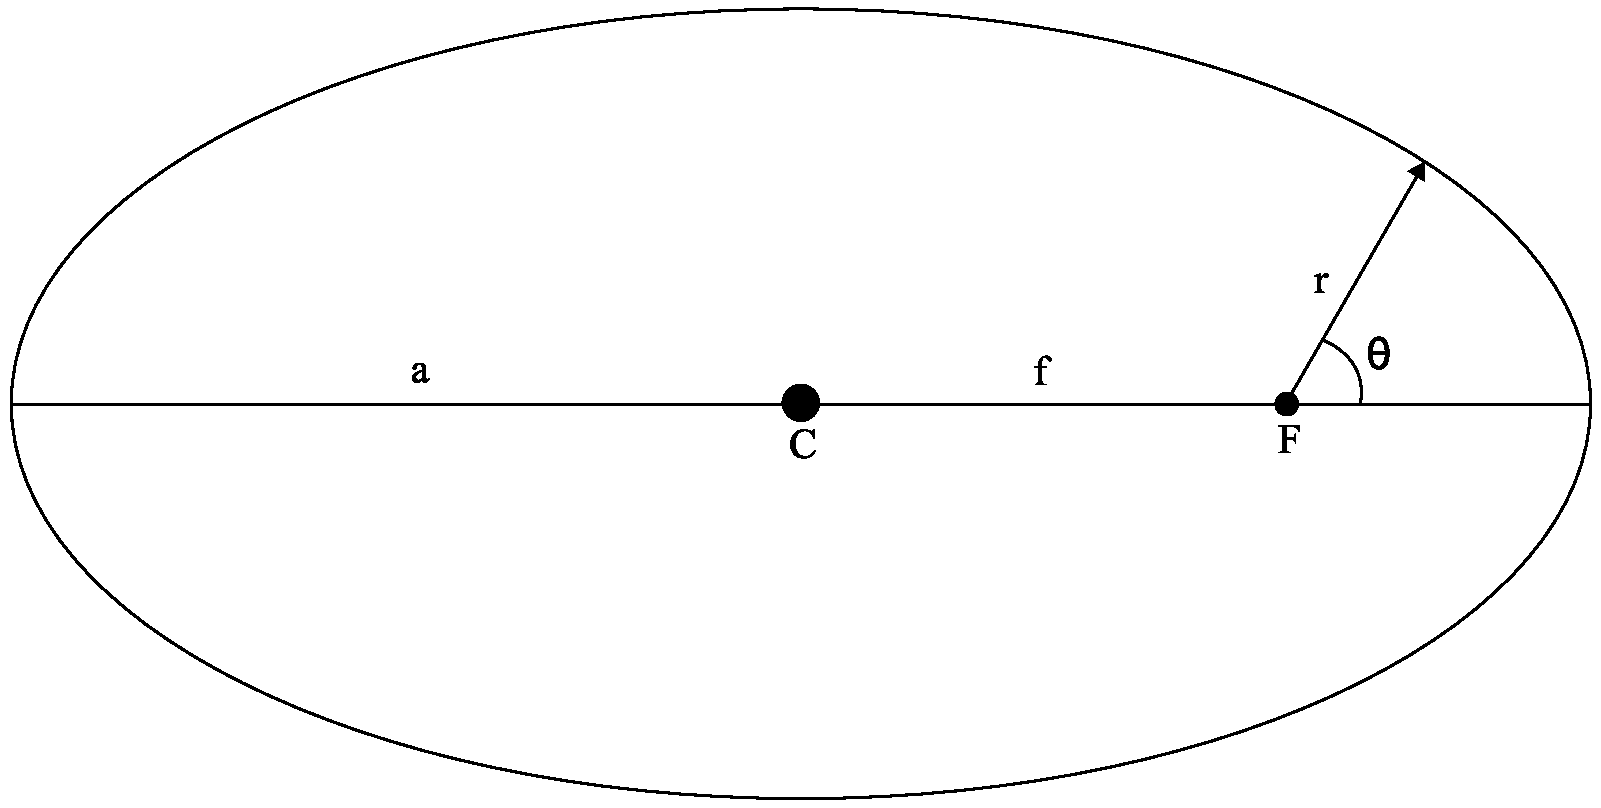
\includegraphics[width=\textwidth]{../images/ellipse.pdf}
\caption{The different parameters of an elliptic orbit. $C$ is the center of the ellipse, $F$ is the main focus of the ellipse, $a$ is the semimajor axis, $f$ is the distance between the center and the focus of the ellipse, $r$ points to the current position of the orbiting body, and $\theta$ is the true anomaly of the object. Eccentricity $e$ can be expressed as the ratio between $f$ and $a$.}
\label{fig:ellipse}
\end{figure}

The solution to the two-body problem works quite accurately for example in our solar system, even though there are more than just two objects. This is because the mass of the Sun dominates all of the interactions and the planets are far away from each other, so each planet can to the first order be examined on its own. However in more extreme environments, the approximation faces some limitations. The singularity in the equation of motion as $r$ approaches 0 is troublesome when running simulations with close encounters, so it is very useful to rewrite the equations so that the singularity doesn't appear. This is called regularization. The equation of motion also works only for classical Newtonian systems, but fails to give correct results when relativistic effects become prominent. Thus the equation must be altered, for example with post-Newtonian terms, to make it applicable in a relativistic setting. The next two chapters tackle these two problems, respectively.

%TODO
%mainitse lopussa että ei toimi täsmälleen tälleen koska suhteellisuusteoria, pohjusta PN hommaa
%koska yhtälöissä on per r termi, tarvitaan regularisaatiota. Menee ikäväksi kun kappaleet ovat hyvin lähellä toisiaan

\section{Regularization}

Because of the $1/r$ term in the equation of motion (equation \ref{equ:eomgravity}), the two-body problem becomes singular when the distance between two objects approaches zero. It is because of these singularities that simulations of the two-body problem become very arduous when collisions or close approaches occur. Integrators may attempt to handle the singularity by taking increasingly smaller time-steps as the separation between the particles decreases, which slows down the entire simulation drastically. The problem can be avoided by transforming to a coordinate system which does not exhibit any singularities, and this procedure is known as regularization \citep{bt-galdyn}. 
%Usually this comes with the cost of having a higher number of variables to keep track of. But regularization shows great advantages in the time-step sizes needed for accurate integration, and the amount of time-steps needed for integrating close encounters is much smaller \citep{diplomarbeit}. 

\subsection{One-dimensional regularization}

The one-dimensional case is simple, but gives a good basis for understanding the methods used in the higher-dimensional cases as well. The Hamiltonian for the relative motion in a one-dimensional two-body problem is
\begin{equation}
H(q,p,t) = K + V = \frac{p^2}{2 \mu} - \frac{G \mu M}{\left| q \right|} \ .
\end{equation}
We may do a transformation to some new coordinate system $(Q, P)$. We can do a canonical point transformation where the old canonical coordinates are changed to new ones through $q = Q^2$. A generating function $S$ is a function, the partial derivatives of which give us the Hamiltonian in the coordinate system. We can now get the new canonical impulses through a generating function of the form
\begin{equation}
S(p,Q) = \sum p q(Q) = pq(Q) = pQ^2
\end{equation}
and
\begin{equation}
P = \frac{\partial S}{\partial Q} = 2pQ \ ,
\end{equation}
so
\begin{equation}
p = \frac{P}{2Q} \ .
\end{equation}
The new Hamiltonian is then
\begin{equation}
H(Q,P,t) = \frac{P^2}{8Q^2 \mu} - \frac{G \mu M}{Q^2} \ .
\end{equation}

Next we want to do a time transformation as well. We may choose a function $t = t(s)$, where $s$ is the new time variable, often also called fictitious or regularized time. In a more general sense we may choose a time transformation function $g(q,p)$ so that $\mathrm{d} t = g \, \mathrm{d} s$ \citep{ad}. For the transformation to remain canonical, our new Hamiltonian must be obtained through the Poincaré time transformation \citep{mikkola:2008}. In the Poincaré transformation one takes time to be a canonical coordinate $(t=q_0)$ and the corresponding momentum of time is the binding energy of the system, $p_0 = -E$. The new Hamiltonian obtained through this transformation is then
\begin{equation}
\Gamma(q,p,s) = g(q,p) (H(q,p,q_0) + p_0) \ .
\end{equation}
By choosing $g = r = \left| q \right| = Q^2$, where $r$ is simply the particle separation, the transformation gives us
\begin{align}
\Gamma(Q,P,s) &= Q^2 \left( \frac{P^2}{8Q^2 \mu} - \frac{G \mu M}{Q^2} -E \right) \nonumber \\
&= \frac{P^2}{8 \mu} - E Q^2 - G \mu M \ .
\end{align}
The canonical equations are now
\begin{align}
\frac{\mathrm{d} Q}{\mathrm{d} s} &= \frac{\partial \Gamma}{\partial P} = \frac{P}{4 \mu} \\
\frac{\mathrm{d} P}{\mathrm{d} s} &= -\frac{\partial \Gamma}{\partial Q} = 2EQ
\end{align}
and give us the equation of motion in these new coordinates
\begin{equation}
\frac{\mathrm{d}^2 Q}{\mathrm{d} s^2} = \frac{E}{2 \mu} Q \label{equ:eomRegu} \ .
\end{equation}
The singularity at $r = 0$ has now been removed. In a bound system $E < 0$, so the solution to the equation of motion is a simple harmonic oscillator.

\subsection{Levi-Civita transformation}

Regularization of the two-dimensional case is quite similar to the one-dimensional case, but now our positions and momentums are two dimensional vectors. It has been named the Levi-Civita transformation, after the Italian mathematician who first used this method \citep{levi-civita:1920}. The Hamiltonian is now
\begin{equation}
H(\mathbf{r},\mathbf{p},t) = \frac{\mathbf{p}^2}{2 \mu} - \frac{G \mu M}{r} \ .
\end{equation}
The transformation to the new coordinates is given via complex numbers. The new coordinates are $Q_1, Q_2$ so that $\mathbf{Q} = Q_1 + iQ_2$ and $r = x + iy = \mathbf{Q}^2 = (Q_1 + iQ_2)^2$. From this we get $x = Q_1^2 - Q_2^2$ and $y = 2Q_1 Q_2$. By again choosing $g = r = \mathbf{Q}^2$ as in the previous section, the Poincaré transform gives us 
\begin{equation}
\Gamma = r \left( \frac{\mathbf{p}^2}{2 \mu} - \frac{G \mu M}{r} - E \right) = \frac{\mathbf{P}^2}{8 \mu} - E \mathbf{Q}^2 - G \mu M \ ,
\end{equation}
where $\mathbf{P} = 2 \mathbf{Q} \cdot \mathbf{p}$. Like in the one-dimensional case, this is the Hamiltonian of a simple harmonic oscillator, except in this case our harmonic oscillator is two-dimensional. The singularity has thus once again been removed.

The transformation $r = \mathbf{Q}^2$ can also be expressed in vector notation as
\begin{equation}
\mathbf{r} = \mathcal{L}(\mathbf{Q}) \mathbf{Q} \ ,
\end{equation}
where $\mathcal{L}(\mathbf{Q})$ is the Levi-Civita matrix
\begin{equation}
\mathcal{L}(\mathbf{Q}) =
\begin{pmatrix}
Q_1 & -Q_2 \\
Q_2 & Q_1
\end{pmatrix} \ .
\end{equation}
This sort of matrix has properties that are useful when formulating transformations in higher dimensional cases.

\subsection{Kustaanheimo-Stiefel method}
While the two-body problem is limited to two dimensions in theory, in practice there are usually perturbations which perturb the orbit into the third dimension, thus a three-dimensional generalization is desirable. A problem with this arises from the fact that it is not possible to do the generalization directly in three dimensions. The Levi-Civita matrix is a good starting point, and it has several useful properties. All of its elements are linear homogeneous functions of $Q_i$, and the mapping defined by the matrix is conformal, i.e. the transformation matrix is orthogonal. A matrix with such properties cannot exist in three dimensions, and the next suitable step from a two-dimensional matrix is a four-dimensional matrix \citep{diplomarbeit}. The Kustaanheimo-Stiefel (KS) method involves doing the transformation into three-dimensional space through four dimensions.

The old and new coordinates are defined as
\begin{align}
\mathbf{Q} &= (Q_1 \ Q_2 \ Q_3 \ Q_4)^\mathrm{T} \nonumber \\
\mathbf{r} &= (r_1 \ r_2 \ r_3 \ r_4)^\mathrm{T} \\
\mathbf{p} &= (p_1 \ p_2 \ p_3 \ p_4)^\mathrm{T}  \nonumber
\end{align}
and the KS matrix is defined as 
\begin{equation}
\mathcal{L}(\mathbf{Q}) =
\begin{pmatrix}
Q_1 & -Q_2 & -Q_3 & Q_4 \\
Q_2 & Q_1 & -Q_4 & -Q_3 \\
Q_3 & Q_4 & Q_1 & Q_2 \\
Q_4 & -Q_3 & Q_2 & -Q_1
\end{pmatrix} \ .
\end{equation}
The transformation is given by the relations 
\begin{equation}
\mathbf{r} = \mathcal{L} \mathbf{Q} \label{equ:KStransform}
\end{equation}
and
\begin{equation}
\mathbf{P} = 2 \mathcal{L}^\mathrm{T} \mathbf{p} \ ,
\end{equation}
and by again using the time transform function $g = r = \mathbf{Q}^2$. Thus we get that
\begin{equation}
\Gamma = r \left( \frac{\mathbf{p}^2}{2 \mu} - \frac{G \mu M}{r} - E \right) = \frac{\mathbf{P}^2}{8 \mu} - E \mathbf{Q}^2 - G \mu M \ ,
\end{equation}
which once again is the Hamiltonian of a harmonic oscillator, this time in four dimensions. The coordinate singularity has again disappeared like in the previous cases.
However there is still an extra dimension, so we need to find a mapping to convert between the three dimensional physical space and the four dimensional space. The simplest way is to set that $r_4 = 0$ and $p_4 = 0$. 

Calculating $\mathbf{r}$ from equation \ref{equ:KStransform} we get
\begin{equation}
\mathbf{r} = 
\begin{pmatrix}
r_1 \\
r_2 \\
r_3 \\
r_4
\end{pmatrix}
=
\begin{pmatrix}
Q_1^2 - Q_2^2 - Q_3^2 + Q_4^2 \\
2(Q_1 Q_2 - Q_3 Q_4) \\
2(Q_1 Q_3 + Q_2 Q_4) \\
0
\end{pmatrix} \ .
\end{equation}
We can still determine one of the extra components of $\mathbf{Q}$, and setting $Q_4 = 0$ gives us the following relations
\begin{align}
Q_1 &= \left( \frac{1}{2} ( r + \left| r_1 \right| ) \right)^{1/2} \nonumber \\
Q_2 &= \frac{1}{2} \frac{r_2}{Q_1} \\
Q_3 &= \frac{1}{2} \frac{r_3}{Q_1} \nonumber \ 
\end{align}
and the mapping
\begin{equation}
\mathbf{Q} = 
\begin{cases}
\left( Q_1 \ Q_2 \ Q_3 \ Q_4 \right)^\mathrm{T} \ , \ \mathrm{if} \ r_1 \geq 0 \\
\left( Q_1 \ Q_2 \ Q_4 \ Q_3 \right)^\mathrm{T} \ , \ \mathrm{if} \ r_1 < 0 \ .
\end{cases}
\end{equation}
With these mappings we can accurately convert the coordinates between the different dimensional spaces \citep{diplomarbeit, ad}.

Regularized computational methods are very precise, but they they are typically much more computationally expensive than non-regularized ones, so there would be benefits for an accurate method that does not need this kind of regularization. Fortunately there exists another method which involves only time transformation but no coordinate transformation, named algorithmic regularization (AR) \citep{diplomarbeit}. These kinds of regularization methods do not actually remove the Newtonian collision singularities from the equations of motion, but the equations can be evaluated in a way that they behave regularly regardless. Algorithmic regularization will be discussed in more detail in chapter \ref{chap:ar-chain}.


%\noindent (TODO: Syvällisemmin KS:ää? Lisää alakohtia? Jonkunlainen loppukaneetti.)

\section{Post-Newtonian dynamics} \label{sect:pndynam}

While Newtonian dynamics is a perfectly valid approximation in everyday life, it stops giving correct results when more massive or faster moving objects are concerned, and instead we need to use general relativity (GR). %TODO Selitä geeärrää?
Doing fully general relativistic simulations is very computationally intensive however, so more wieldy methods are required for large-scale simulations. This is where post-Newtonian (PN) expansions come in. Post-Newtonian expansions in general relativity are used for finding an approximate solution of the Einstein field equations for the metric tensor. %TODO selitä noi lisäks
Einstein field equations are the set of 10 equations in Albert Einstein's general theory of relativity that describe the fundamental interaction of gravitation as a result of spacetime being curved by mass and energy.
%TODO tää kopipastattiin aiemmas
In other words, the post-Newtonian theory is an approximate version of general relativity that applies when the gravitational field is relatively weak, and the motion of the matter is slow. The theory successfully describes the gravitational field of our solar system, but it can also be applied to situations involving compact bodies with strong internal gravity.
%provided that the mutual gravity between bodies is weak enough.

%
%The post-Newtonian theory is derived from the Landau-Lifshitz formulation of the Einstein field equations. The equations can be written as 
%\begin{equation}
%\partial_{\mu \nu} H^{\alpha \mu \beta \nu} = \frac{16 \pi G}{c^4}(-g)(T^{\alpha \beta} + t^{\alpha \beta}_{LL}) \ ,
%\end{equation}
%where $H^{\alpha \mu \beta \nu} \equiv \mathfrak{g}^{\alpha \beta} \mathfrak{g}^{\mu \nu} - \mathfrak{g}^{\alpha \mu} \mathfrak{g}^{\beta \mu}$ is a tensor density which possesses the same symmetries as the Riemann tensor. In the Landau-Lifshitz formulation the main variables are not the components of the metric tensor $g_{\alpha \beta}$, but those of the gothic inverse metric $\mathfrak{g}^{\alpha \beta} \equiv \sqrt{-g} g^{\alpha \beta}$, where $g^{\alpha \beta}$ is the inverse metric, and $g$ the metric determinant. $T^{\alpha \beta}$ is the energy-momentum tensor of the matter source term, and the Landau-Lifshitz pseudotensor $(-g) t^{\alpha \beta}_{LL} \sim \partial \mathfrak{g} \cdot \partial \mathfrak{g}$ can be interpreted as an energy-momentum (pseudo)tensor for the gravitational field.
%
%The antisymmetry of $H^{\alpha \mu \beta \nu}$ implies the conservation equation
%\begin{equation}
%\partial_\beta \left[ (-g)(T^{\alpha \beta} + t^{\alpha \beta}_{LL}) \right] = 0 \ ,
%\end{equation}
%which is formally equivalent to $\nabla_\beta T^{\alpha \beta} = 0$, where $\nabla_\beta$ is the covariant derivative operator. The conservation equation allows for the formulation of global conservation laws, for example for energy, linear momentum, and angular momentum. We then introduce the gravitational potentials $h^{\alpha \beta} = \eta^{\alpha \beta} - \mathfrak{g}^{\alpha \beta}$, where $\eta^{\alpha \beta} = diag(-,+,+,+)$ is the Minkowski metric expressed in Lorentzian coordinates, and impose the harmonic coordinate gauge condition $\partial_\beta h^{\alpha \beta} = 0$.
%
%The field equations become a wave equation in flat spacetime
%\begin{equation} \label{equ:waveeq}
%\square h^{\alpha \beta} = -\frac{16 \pi G}{c^4} \tau^{\alpha \beta} \ ,
%\end{equation}
%where $\square = -\frac{1}{c^2} \frac{\partial^2}{\partial t^2} + \frac{\partial^2}{\partial x^2} + \frac{\partial^2}{\partial y^2} + \frac{\partial^2}{\partial z^2}$ is the flat spacetime d'Alembert operator, and $\tau^{\alpha \beta} = (-g)(T^{\alpha \beta} + t^{\alpha \beta}_{LL} + t^{\alpha \beta}_H)$ is defined as the effective energy-momentum pseudotensor, composed of a matter contribution, the Landau-Lifshitz contribution, and the harmonic gauge contribution $t^{\alpha \beta}_H \sim \partial h \cdot \partial h + h \partial^2 h$. The conversation equation now reads $\partial_\beta \tau^{\alpha \beta} = 0$.
%
%So far no approximations have been made, and the wave equation combined with the harmonic gauge condition and conservation equation is an exact formulation of the Einstein field equations. The wave equation determines the potential $h^{\alpha \beta}$ for a given distribution of matter. The behaviour of the matter is determined by the conservation equation/gauge condition.
%
%The wave equation can be integrated without enforcing the conservation equation, and this is known as the relaxed Einstein field equations. The integration is achieved by iteration. Assuming that $h^{\alpha \beta}_n$ is known, $h^{\alpha \beta}_{n+1}$ is obtained by solving
%\begin{equation}
%\square h^{\alpha \beta}_{n+1} = -\frac{16 \pi G}{c^4} \tau^{\alpha \beta}[h_n] \ .
%\end{equation}
%The iterations are started with $h^{\alpha \beta}_0 = 0$, and stopped when the desired accuracy is obtained. In principle, the truncation is the only source of approximation. The procedure produces a formal expansion of $h^{\alpha \beta}$ in powers of G. This is known as the post-Minkowskian expansion of the gravitational field. After iterations have been done up to the desired accuracy, we can again impose the gauge condition to get a proper metric.

%The difference between post-Minkowskian and post-Newtonian expansion is that in post-Newtonian approximation we assume a slow-motion condition, i.e. all speeds within the matter distribution (such as the speed of sound within a body, or the speed of the body as a whole) are small compared with the speed of light. In astrophysical situations the assumption of slow speeds is accurate in the vast majority of cases, since the virial theorem implies that $U \sim v^2$ for any gravitationally bound system; weak fields are naturally accompanied by slow motion.



The approximations are expanded in small parameters which express orders of deviations from Newton's laws of gravity. A correction of order $(v/c)^n$ to a Newtonian expression is said to be of $\mathrm{PN}(n/2)$ order.

The first use of a PN expansion (to first order) was made by Einstein in calculating the perihelion precession of Mercury's orbit.
Mercury's perihelion precesses (rotates) around the sun. This is mainly due to perturbations caused by the presence of the other planets. Another much less significant factor is the oblateness of the sun. In the 1800s it was noticed that the orbit deviates from the precession predicted by these Newtonian effects by about 43 arc seconds per a tropical century.

Several different reasons for this deviation were proposed, and perhaps the most prevalent of these was Vulcan. Vulcan is a small hypothetical planet that was supposed to orbit the sun inside the orbit of Mercury. The perturbations caused by this planet could have explained the anomalous precession of Mercury. The existence of the planet was hypothesized by the French mathematician Urbain Le Verrier, who also predicted the existence and position of Neptune with only mathematics. While many people claimed to have observed the planet, its supposed orbit was so close to the sun that this was extremely challenging to verify.

There were attempts to confirm the existence of the planet, but in 1915 the hypothetical planet was quite firmly put to rest when Einstein explained the anomalous precession through his theory of relativity. The reason why the same extra precession that affects all of the planets had been observed only with Mercury is that the magnitude of the differences from simple Newtonian theory diminishes rapidly as one gets farther from the Sun. Mercury's fairly eccentric orbit also makes it much easier to detect the perihelion shift than is the case for the nearly circular orbits of Venus and Earth.
This was the first case of solving the general relativistic two-body problem, which is the most common use of the PN expansion nowadays. %TODO Lisää hommaa, toimii myös aurinkokunnassa, referenssejä Vulkanukseen wikipediasta

%Hyvää matskua: gravity postminkowskian implementation sivu 10, gravity postnewtonian fundamental heti alku, common reader 3.2

In the case of a two-body system, the post-Newtonian corrections give rise to a perturbed Keplerian orbit. The only secular effect on the orbit is the pericenter advance.
PN1 terms are the ones responsible for the advance of the pericenter of an eccentric orbit, given by $\dot{\omega} = 6 \pi f_\mathrm{b} m/a (1-e^2)$, where $a$ and $e$ are the semimajor axis and eccentricity of the orbit, and $f_\mathrm{b}$ is the orbital frequency, given by Kepler's third law $2 \pi f_\mathrm{b} = (m/a^3)^{1/2}$ \citep{will:2006}. 

The intrinsic angular momentum (spin) of a body is also a source of gravity that affects the metric and body motions. The spin causes precession in the ascending node. %TODO lisää kaavaa, gravity kalvoista

There are some systems that cannot be properly described by post-Newtonian approximation because of their extreme conditions. Some examples of such systems include the final phases of a compact object merger, the cores of supernovae, and the structure of rapidly rotating neutron stars. These must be analysed using different methods, for example the full solution of Einstein's equations via numerical methods \citep{will:2006}. 

\section{Black holes in galaxy mergers}

\section{Black hole mergers}
\subsection{Dynamical friction}
\subsection{Three body scattering}
\subsection{Gravitational waves}

\chapter{AR-CHAIN} \label{chap:ar-chain}
\section{AR-CHAIN overview}

The code uses post-Newtonian corrections to take into account and approximate the relativistic effects near the black hole particles. The corrections are represented by additional terms in the relative accelerations of the two bodies, so that
\begin{equation}
\boldsymbol{a}_\mathrm{2-body} = \boldsymbol{a}_\mathrm{Newtonian} + \sum_{k=2}^7 c^{-k} \boldsymbol{a}_\mathrm{(k/2)PN} + \boldsymbol{a}_S \ ,
\end{equation}
where $\boldsymbol{a}_\mathrm{Newtonian}$ is the usual Newtonian two-body acceleration, $c$ is the speed of light, $\boldsymbol{a}_\mathrm{xPN}$ is the PN correction of order $x$, and $\boldsymbol{a}_S$ indicates PN terms depending on the spins of the particles. PN corrections up to order PN3.5 are included in the code.

For spinning bodies, additional PN corrections are required. The PN contribution to the equations of motion for the spins is given by
\begin{equation}
\boldsymbol{\dot{S}}_i = \boldsymbol{S}_{\mathrm{PN},i} \times \boldsymbol{S}_i \ ,
\end{equation}
where $\boldsymbol{S}_i$ is the spin angular momentum of the particle $i$ and $\boldsymbol{S}_{\mathrm{PN},i}$ gives the effect of the spin-orbit, spin-spin, and quadrupole-monopole interactions. %TODO Selitä näitä pls

These two-body PN corrections are only used when at least one of the bodies is a black hole, since for other particles they're not of any significance. Only when a black hole is involved are the velocities and masses large enough to require relativistic treatment.

\section{Bulirsch–Stoer algorithm}
\section{Time-transformed leapfrog}
\section{Collisions}

\chapter{AR-CHAIN results}
\section{OJ287}

These following runs all had similar initial conditions, apart from the magnitude of the spin. The initial values for the orbital elements were those measured by Valtonen \& Mikkola (cite), with the semimajor axis of the binary being around 11350 AU, the eccentricity being 0.6, and spin being 0.28. Simulations were also run with a spin of 0 and a spin three times the original. The direction of the spin was towards the positive z-axis of the system. The inclination of the orbit was 45 degrees in the xz-plane. So the spin was inclined 45 degrees to the initial orbit. The initial timestep in the simulations was 0.01 gadget times, and the interval for writing the data in a file was 1 gadget time. 

The orbital elements precessed, so average values were used to make smoother and clearer graphs. 

The eccentricity of the orbit goes down as the orbit circularizes due to the GW emissions.

The PN2.5 term is responsible for the GW emissions.

The spin caused the orbit to twist. This can be seen clearly in images \ref{fig:spin0Orbits} and \ref{fig:spinNormalOrbits}. If there was no spin, the orbit stayed neatly in the original plane, but with spin the orbit started turning.

One should keep in mind that this model is very simplistic. There are only the two black holes, and no other stars to interact with, and no accretion disks, which are thought to play a relatively large role in the life of the system.

\begin{figure}[h!tb]
\centering
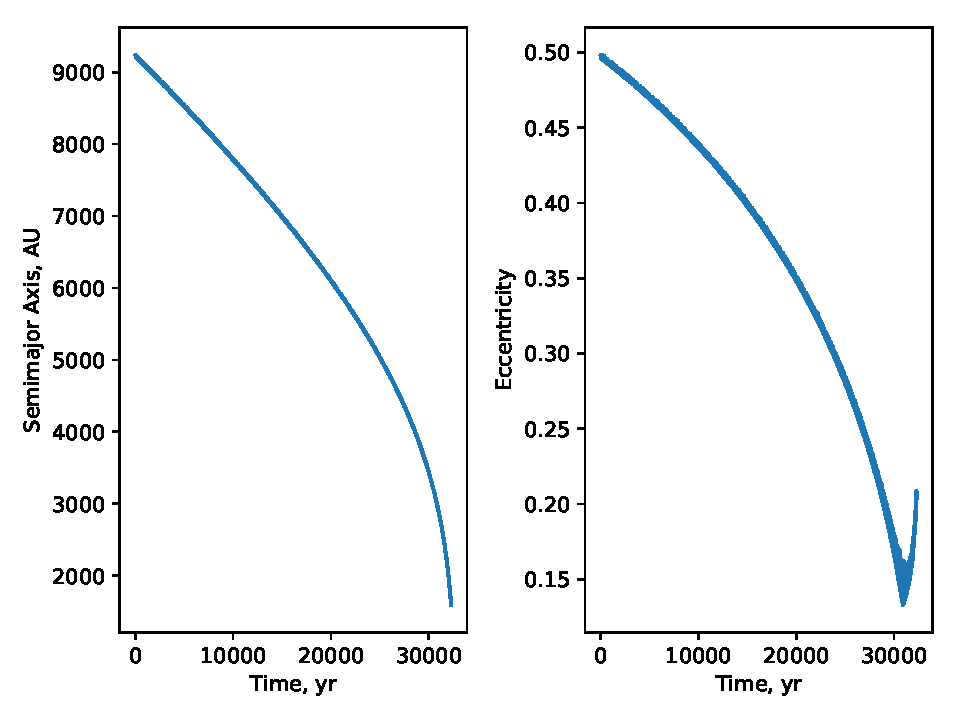
\includegraphics[width=\textwidth]{../images/spinNormal.pdf}
\caption{The development of the semimajor axis and eccentricity of the smaller of the two black holes in the binary, with it having a spin of 0.28. The merging happened at around 206800 gadget time, corresponding to 32300 years.}
\label{fig:spinNormal}
\end{figure}

\begin{figure}[h!tb]
\centering
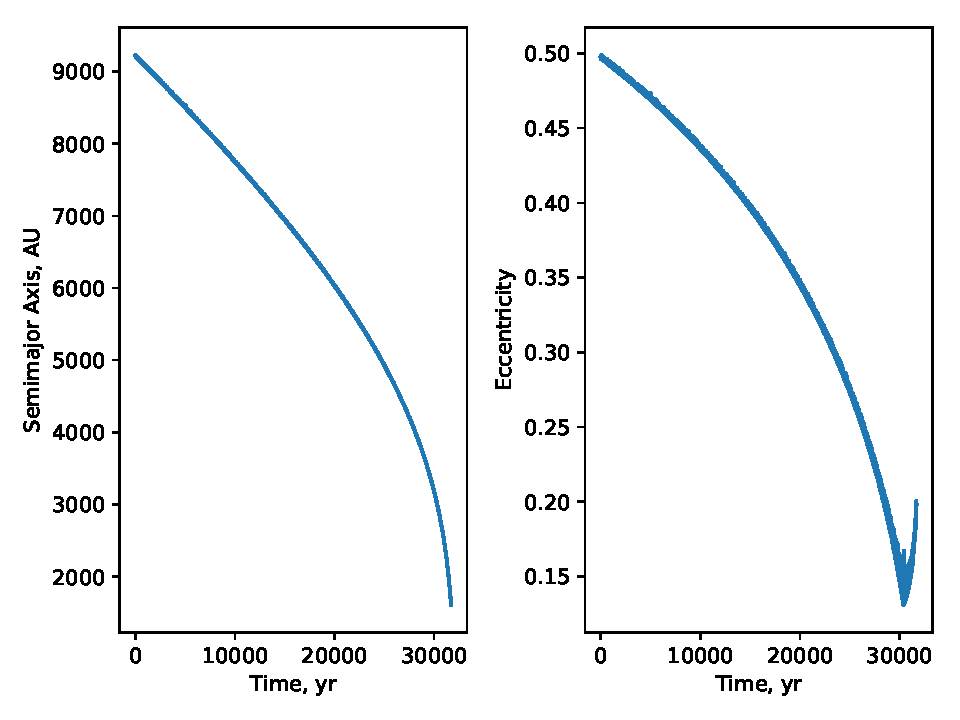
\includegraphics[width=\textwidth]{../images/spin0.pdf}
\caption{The development of the semimajor axis and eccentricity of the smaller of the two black holes in the binary, with it having no spin at all. The merging happened at around 202300 gadget time, corresponding to 31700 years.}
\label{fig:spin0}
\end{figure}

\begin{figure}[h!tb]
\centering
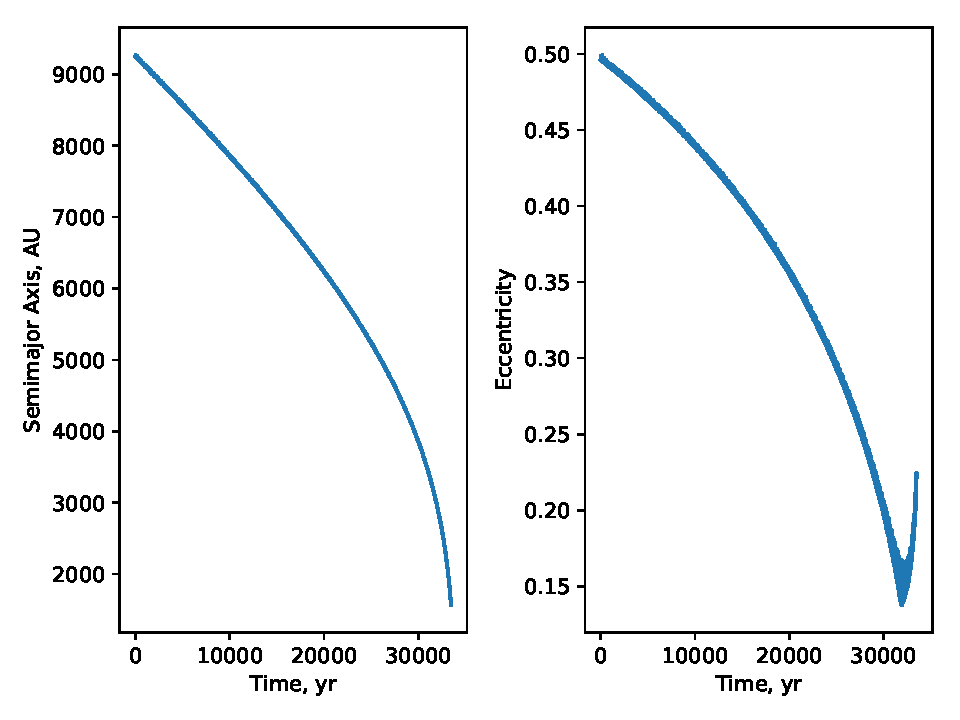
\includegraphics[width=\textwidth]{../images/spin3.pdf}
\caption{The development of the semimajor axis and eccentricity of the smaller of the two black holes in the binary, with it having a spin of 0.84, three times the real value. The merging happened at around 214400 gadget time, corresponding to 33500 years.}
\label{fig:spin3}
\end{figure}

\begin{figure}[h!tb]
\centering
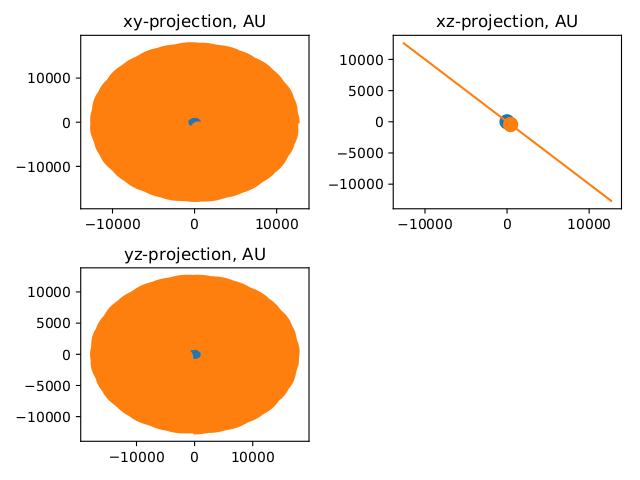
\includegraphics[width=\textwidth]{../images/spin0Orbits.png}
\caption{Plot of the the orbits of the binary if there is no spin. The orbiting member doesn't leave the original plane it was in.}
\label{fig:spin0Orbits}
\end{figure}

\begin{figure}[h!tb]
\centering
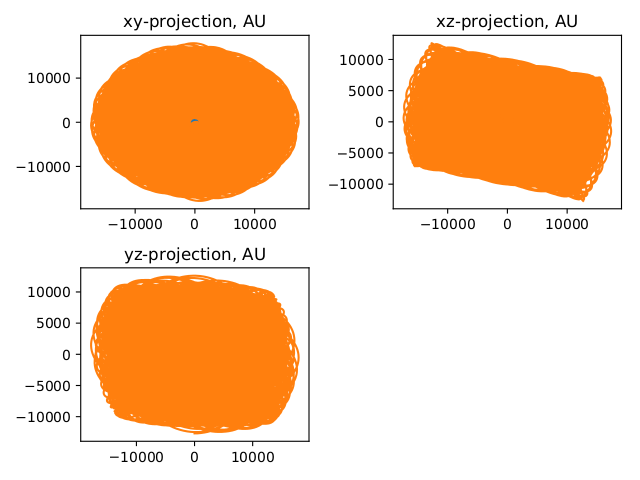
\includegraphics[width=\textwidth]{../images/spinNormalOrbits.png}
\caption{Plot of the the orbits of the binary with the measured spin.}
\label{fig:spinNormalOrbits}
\end{figure}

\begin{figure}[h!tb]
\centering
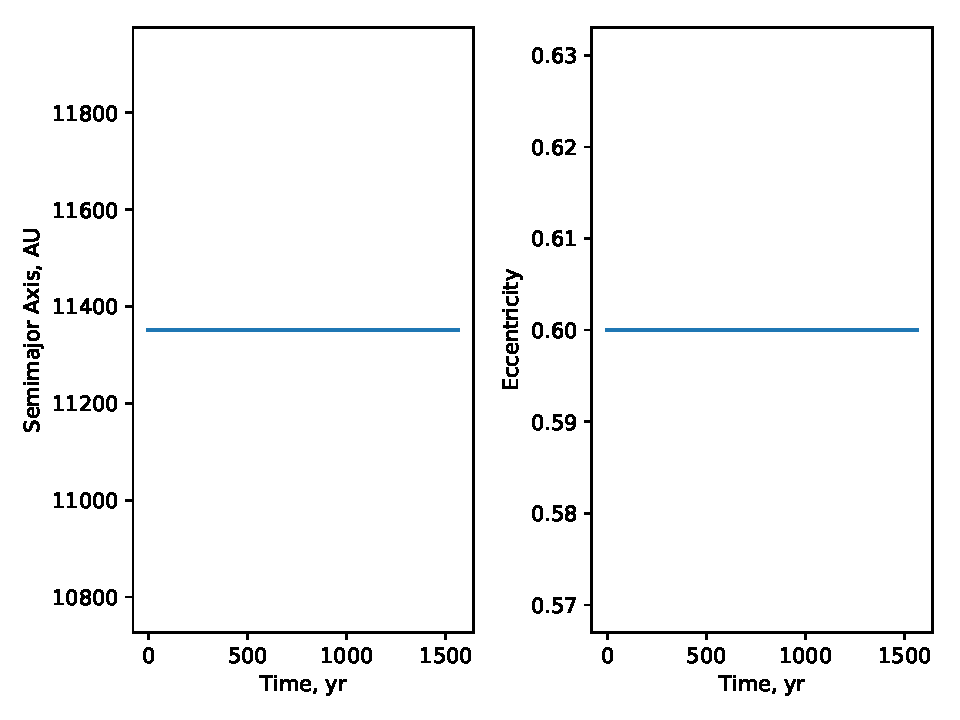
\includegraphics[width=\textwidth]{../images/noPN.pdf}
\caption{The development of the semimajor axis and eccentricity of the smaller of the two black holes in the binary, if the post-Newtonian terms aren't factored in. The simulation was run for slightly over 1500 years. Since the PN terms were not taken into account the orbit didn't actually decay, just as expected. The results themselves aren't very interesting, but it shows that the corrections are indeed needed for realistic results.}
\label{fig:noPN}
\end{figure}

\subsection{Estimated time of merging}
\subsection{Differences from reality}
\section{Effects of spin}

\chapter{KETJU and results}
\section{KETJU overview}
\section{}
\section{}

\chapter{Conclusions}

% STEP 5:
% Uncomment the following lines and set your .bib file and desired bibliography style
% to make a bibliography with BibTeX.
% Alternatively you can use the thebibliography environment if you want to add all
% references by hand.

\clearpage
\addcontentsline{toc}{chapter}{Bibliography} % This lines adds the bibliography to the ToC
\bibliographystyle{plainnat}
\small
\bibliography{lahteet}


\end{document}

